\chapter{Using a Do file}
\graphicspath{ {./Lab00HowTo/howTo30 Using Do Files/Fig} }

I find setting up the testbench waves to be a pain, especially when you
are making a lot of mistakes and need to rerun your simulation multiple
times; each time setting up the waveforms. In order to simplify the
process of setting up the waveforms, you can write a script files that
performs the waveform setup and then call the script file inside
ModelSim. The script file is called a ``do'' file. They are very easy to
make and will save you time. If a do file is provided to you, you will
most likely need to edit it because your signal names may be different.

In the discussion below I have used two placeholders:
\file{<labName>} is the name of your testbench module.
\file{<projectDirectory>} is the system path to your
Verilog files corresponding to your project.

\begin{itemize}
    \item
        If provided, download  \file{<labName>\_tbWaveSetup.do} into the:

        \file{<projectDirectory>\textbackslash simulation\textbackslash modelsim} directory
        If this folder does not exit, then you need to have to run
        ``Start Analysis and Elaboration'' at least once. You will know you are in
        \file{<projectDirectory>} when you see the project QPF file.

    \item
        If a do file is not created, you can use the template provided in
        Listing~\ref{listing:howToDoFile} as a starting point to make one
        for yourself. Make sure to put the do file in the:

        \file{<projectDirectory>\textbackslash simulation\textbackslash modelsim} directory
    \item
        Open \file{<labName>\_tbWaveSetup.do} file using Notepad.
        The syntax is pretty straight forward and corresponds to the text
        displayed in the ModelSim console window when you add or modify
        waveforms.
    \item
        From Quartus, you need to:

        \begin{itemize}
            \item
                Make sure that your testbench is the top-level. Do this in the
                Project Navigator, select File view and then right click on the file
                testbench and select ``Set As Top Level Entity''
            \item
                Launch the simulation. Do this by selecting Tools -\> Run Simulation Tool -\> RTL Simulation
            \item
                This will launch Model Sim for your testbench
        \end{itemize}
    \item
        From Model Sim, you need to:

        \begin{itemize}
            \item
                Maximize the Model Sim window -- this makes it easier to see all the
                subwindows.
            \item
                In the library subwindow, open the \textbf{work} library
            \item
                Right click on your testbench and select Simulate
            \item
                In the console area of ModelSim (shown in the image below) type:
        \end{itemize}

\begin{verbatim}
VSIM 3> do  <projectName>\_tbWaveSetup.do
\end{verbatim}

        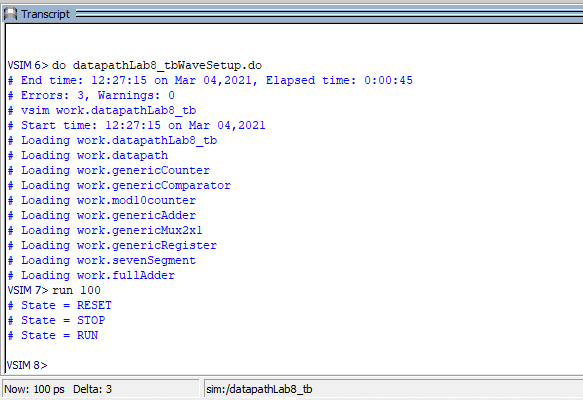
\includegraphics[width=0.4\paperwidth]{image1.png}

    \item
        You can type ``run \textless time\textgreater'' in this area (as
        shown) to simulate some amount of time. I found this VERY handy when
        debugging my Verilog code.
    \item
        Also note that the console has tab completion. This allows you to type
        the first few characters of a command/filename and press Tab to fill
        in the rest of the command/filename. If there is more than one choice,
        the command/filename will be completed up to the ambiguity.
\end{itemize}

\section{Example do file for hiLow Module}

\begin{itemize}
    \item
        Run the testbench for the hiLow module provided on Canvas. Produce a
        timing diagram with the following characteristics. Zoom to fill the
        available horizontal space with the waveform. Color inputs green and
        outputs red. Order the traces from top to bottom as

        \begin{tabular}{p{4cm}p{4cm}p{4cm}}
            signal & radix & color trace \\ \hline
            t\_seedSwitch     &    unsigned     & green \\
            t\_guessSwitch     &    unsigned     & green \\
            t\_playSwitch     &     unsigned     & green \\
            t\_randBut     &     default     & green \\
            t\_hiLowBut     &    default     & green \\
            LFSR         &     unsigned     & yellow\\
            t\_randNum     &    hex         & red \\
            t\_randDisp     &     hex         & red \\
            t\_hiLowSeg     &    hex         & red \\
            t\_greenLEDs     &    default     & red \\
        \end{tabular}

    \item
        The do file for this testbench is shown in Listing~\ref{listing:howToDoFile}. From top to
        bottom the sections are as follows.

        \begin{itemize}
            \item
                Any line that starts with a ``\#'' is a comment. The URL is a
                complete reference for do file syntax.
            \item
                The restart command resets the simulation. I included this because I
                sometimes like to rerun the same simulation multiple times. This
                isn't particularly useful for combinational logic circuits.
            \item
                The delete wave command removes any waveforms that may have been
                added previously. Again, I included this because I sometimes like to
                rerun the same simulation multiple times
            \item
                The add wave command puts a signal into the waveform viewing area.
                There are two parameters included which you will find helpful.

                \begin{itemize}
                    \item
                        Radix changes what base the waveform value is displayed.
                    \item
                        Color changes the color that the waveform is displayed.
                \end{itemize}
        \end{itemize}
    \item
        Once you have created the do file, you call it by running it from the
        console area using the do command discussed previously.
    \item
        You can advance the simulation time using the run command discussed
        previously.
\end{itemize}

\begin{lstlisting}[language=tcl,
caption={do file for  hiLow\_tb.},
label={listing:howToDoFile},
basicstyle=\tiny,
frame=single]

####################################################################
#File:    hiLow_tbWaveSetup.do
####################################################################
restart -f
delete wave *

add wave -position end  -radix unsigned -color green sim:/hiLow_tb/t_seedSwitch
add wave -position end  -radix unsigned -color green sim:/hiLow_tb/t_guessSwitch
add wave -position end  -radix unsigned -color green  sim:/hiLow_tb/t_playSwitch
add wave -position end  -color green sim:/hiLow_tb/t_randBut
add wave -position end  -color green sim:/hiLow_tb/t_hiLowBut
add wave -position end  -radix unsigned -color yellow sim:/hiLow_tb/uut/randNum
add wave -position end  -radix hex -color red sim:/hiLow_tb/t_randDisp
add wave -position end  -radix hex -color red sim:/hiLow_tb/t_hiLowSeg
add wave -position end  -color red sim:/hiLow_tb/t_greenLEDs

    \end{lstlisting}

\section{Model Sim commands}
ModelSim macros (also called DO files) are scripts that contain ModelSim and, optionally, Tcl commands.

You run the commands by typing tyhem in the console window at the bottom of the ModelSim window.
What follows are the most popular commands that we use in the class.  This is not an exhaustive list.
You can find the complete list of command in the
\file{ModelSim® Command Reference Manual} pdf.  You will have to search
the internet for this file as its location changes.

\begin{description}
    \item[do \file{<file>}] The do command executes commands contained in a macro \file{<file>}.
        If you provide no argument, the simulation runs for the default time (100 ns).

    \item[run <time>]This command advances the simulation by the specified <time>.

    \item [restart] This command retarts the simuloation and resets the simulation time to zero.
        The -f option specifies that the simulation will be restarted without requiring confirmation in a
        popup window.

    \item[delete wave] This command removes waveforms from the Wave window.  The * option
        removes all the waves.

    \item[add wave] This command can add signals, waves and busses to the Wave window:
        \begin{itemize}
            \item -position Specifies where the command adds the signals.
            \item  -radix Specifies a user-defined radix.
            \item  -color Specifies the color used to display a waveform.
        \end{itemize}

    \item [radix define] This command is used to create a user-defined radix used to
        map bit patterns to a set of enumeration labels.  This command is used to map the
        binary codes for the states in a finite state machine (FSM) into symbolic names that are
        displayed on the timing diagram.  This makes it much easier to understand what
        state your FSM is in.  This bit patterns may contain ``?'' as a don't care specifier.

    \item[vsim \file{<testbench>}] This eliminates the need to open the word library and simulate the testbench.
        This is a legacy command that is no longer used in the class, until you see it.

\end{description}
